\begin{frame}
    \begin{center}
        \vspace{3.0cm}
        \normalsize
        \textbf{Игровые программы.\\Основы проектирования.} \\
        \vspace{1.4cm}
        \raggedleft\small\textbf{Выполнил:}\\Голубев~А.~В.\\САПР-1.1п\\
        \vspace{1.4cm}
        \vspace{\fill}
        \centeringВолгоград \the\year
    \end{center}
\end{frame}

\begin{frame}
    \frametitle{Цели и задачи проекта}

    \emph{Целью создания} системы являются:
    \begin{itemize}
        \item разработка электронного методического пособия по разработке структуры игровой программы
        \item создание игрового приложения базирующееся на данной структуре
    \end{itemize}

    Основным \emph{функциональным назначением} системы являются:
    \begin{itemize}
        \item представление базовой структуры в проектировании игровых программ
        \item ознакомление с основными алгоритмами используемыми в разработке
        \item предоставление студенту базовых знаний работы с SDL2, SDL2 image, 
            OpenAL, libvorbis
    \end{itemize}
\end{frame}

\begin{frame}
    \frametitle{Описание объекта автоматизации}
    \emph{Объектом автоматизации} является процесс разработки игровых программ.

    \emph{Автоматизация процесса} состоит в следующем:
    \begin{itemize} 
        \item использовании методического пособия для разработки игрового приложения
        \item предоставление справочной информации по разработке компонентов системы
        \item организации взаимодействия между компонентами системы
    \end{itemize}
\end{frame}

\begin{frame}
    \frametitle{Функциональная структура АС}
    Функциональная структура разработанной системы может быть представлена в следующем виде:
    \begin{figure}
        \centering
        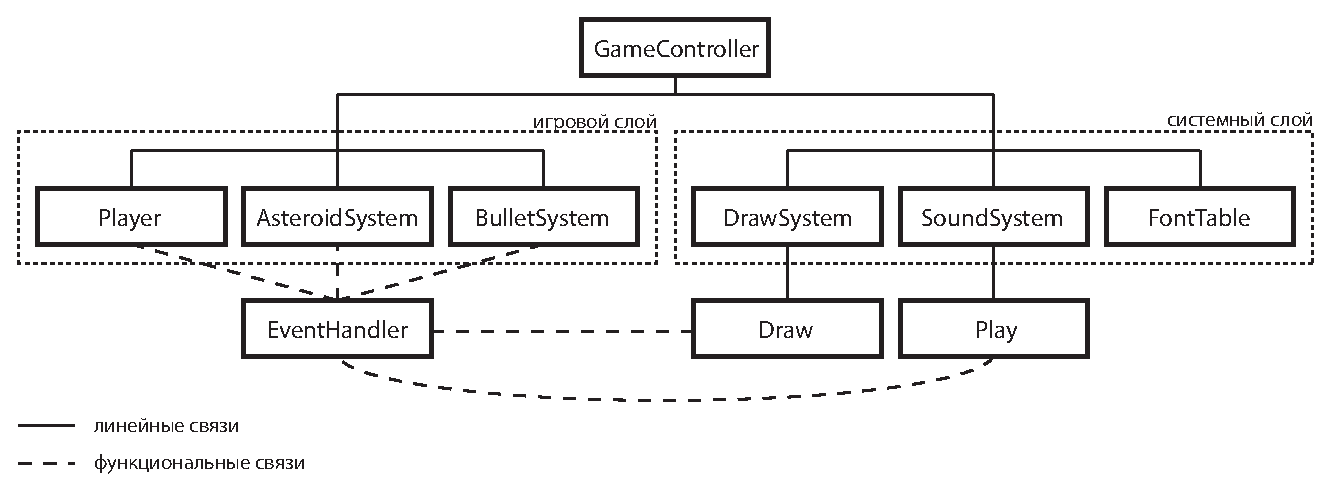
\includegraphics[width=1.0\textwidth]{functional_system}
    \end{figure}
    с разделение игровой программы на два слоя:\\
    --- игровой \qquad --- системный\\
\end{frame}

\begin{frame}
    \frametitle{Функциональная структура АС}
    Более подробная структура взаимодействия между системами:
    \begin{figure}
        \centering
        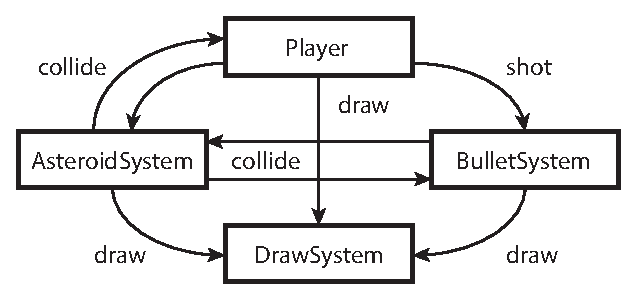
\includegraphics[width=1.0\textwidth]{system_handler}
    \end{figure}
\end{frame}

\begin{frame}
    \frametitle{Описание входных и выходных данных АС}

    \emph{Входные данные}:
    \begin{itemize}
        \item загружаемые ресурсы\\
        \scriptsize изображения, аудио, файлы конфигурации
        \item \normalsize действия пользователя\\
        \scriptsize управление персонажем с помощью клавиатуры
    \end{itemize}
    \emph{Выходные данные}:
    \begin{itemize}
        \item реакция игровой логики\\
        \scriptsize обработка столкновений, воспроизведение звуков, подсчёт очков и т.д.
        \item \normalsize графическая визуализация\\
        \scriptsize представление игровых объектов, очков и количества жизней
    \end{itemize}
\end{frame}

\begin{frame}
    \frametitle{Логическая структура АС}
    Логическая структура автоматизированной системы может быть представить в следующем виде:
    \begin{figure}
        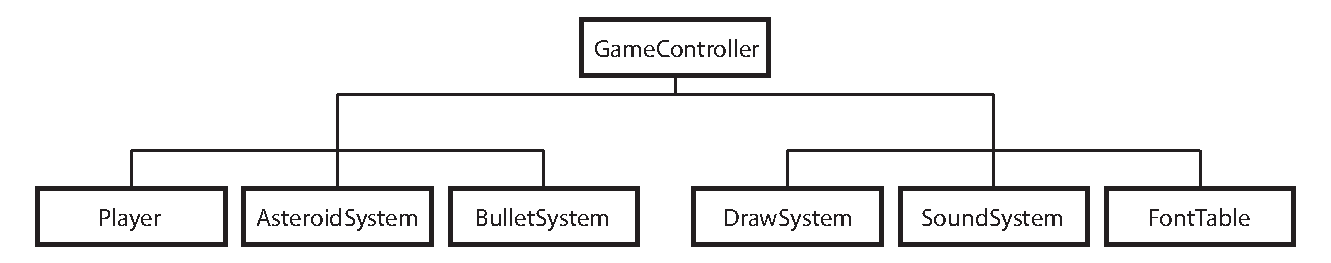
\includegraphics[width=1.0\textwidth]{logic_struct}
    \end{figure}
    \begin{itemize}
        \small
        \item \emph{GameController} -- управляющая программа
        \item \emph{Player} -- управляемый корабль
        \item \emph{AsteroidSystem} -- система астероидов
        \item \emph{BulletSystem} -- система снарядов
        \item \emph{DrawSystem} -- графическая система
        \item \emph{SoundSystem} -- звуковая система
        \item \emph{FontTable} -- загрузка и рисование шрифта
    \end{itemize}
\end{frame}

\begin{frame}
    \frametitle{Архитектура АС}
    \begin{figure}
        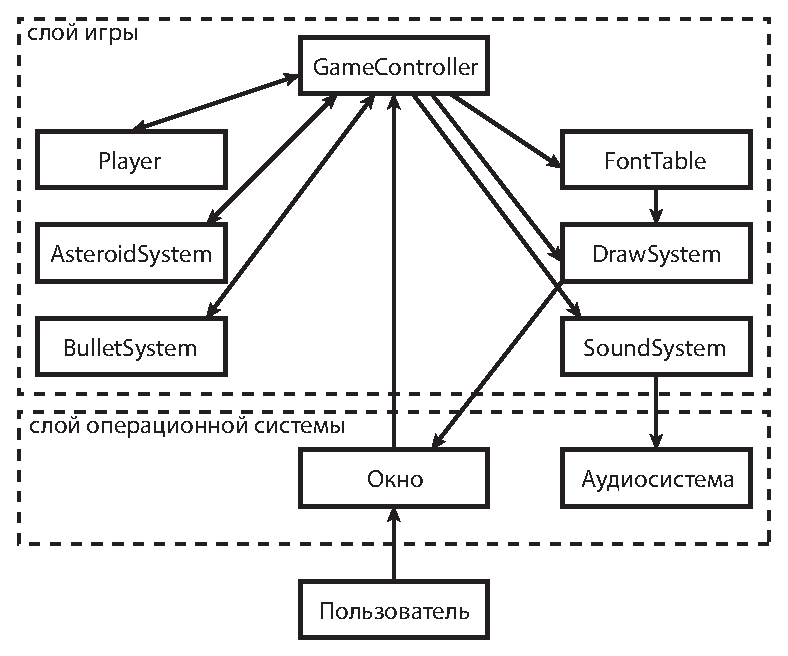
\includegraphics[width=0.85\textwidth]{arch_system}
    \end{figure}
\end{frame}

\begin{frame}
    \frametitle{Выводы}

    В ходе курсовой работы было сделано следующее:
    \begin{itemize}
        \item написано руководство по разработке игровой программы
        \item описаны алгоритмы используемые в разработке
        \item реализованы системы описанные в ТЗ
        \item разработана игровая программа
        \item произведена сборка и тестирование игровой программы
    \end{itemize}

    \vspace*{3em}
    Исходный код доступен по следующей ссылке: \scriptsize
    \url{https://github.com/FreeCX/study/tree/master/cad-fac/it/game/02_minimal}
\end{frame}

\begin{frame}
    \frametitle{Приложение А: скриншоты программы}
    \begin{figure}
        \begin{minipage}{0.49\textwidth}
            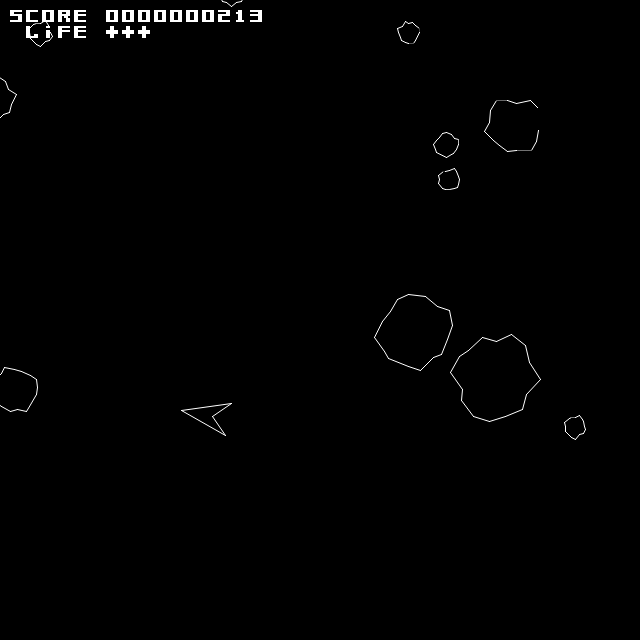
\includegraphics[width=1.0\textwidth]{scrshot01}
        \end{minipage}
        \begin{minipage}{0.49\textwidth}
            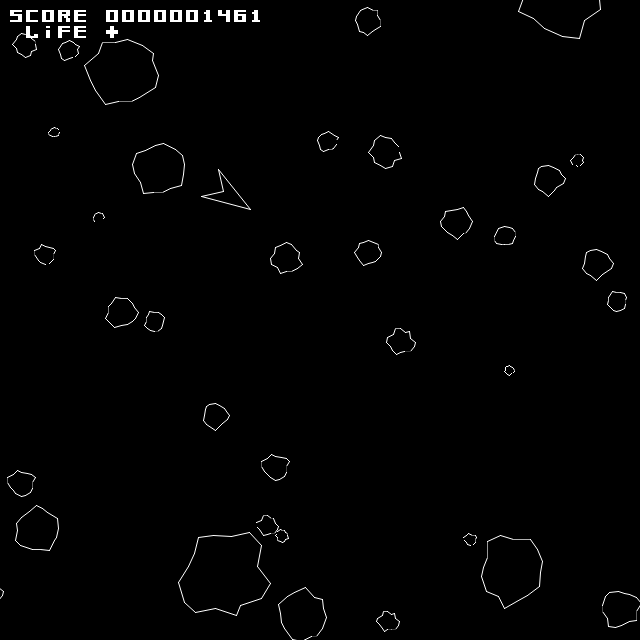
\includegraphics[width=1.0\textwidth]{scrshot02}
        \end{minipage}
    \end{figure}
\end{frame}